\subsection{Sensors}

\subsubsection{Landmine Detection Techniques}

Landmine detection technologies have evolved to encompass a wide range of sensing principles, each targeting specific physical, chemical, or biological characteristics of surface-laid and buried mines. Broadly, these methods can be categorized into five general classes: \textit{\textbf{electromagnetic induction-based} techniques}, \textit{\textbf{radiowave and microwave-based} systems}, \textit{\textbf{mechanical and vibro-acoustic} methods}, \textit{\textbf{spectral and thermal imaging} approaches}, and \textit{\textbf{chemical and biological} sensing methods}. Within each class, a variety of specialized detection technologies have been developed, including traditional metal detectors, ground-penetrating radar, infrared and hyperspectral imaging, seismic/acoustic sensors, vapor detection, and biosensors. Each of these approaches offers distinct advantages and faces specific limitations, especially when adapted to drone-based platforms for remote and efficient minefield scanning. In the following subsections, each class is explored in detail, with emphasis on the operating principles, detection capabilities, challenges, and documented UAV-based applications.

\paragraph{Electromagnetic Induction-Based Techniques}

Electromagnetic induction (EMI) methods operate by exploiting the interaction between electromagnetic fields and conductive or magnetic materials in the ground. These systems are typically composed of a transmitter coil that emits a time-varying electromagnetic field into the soil. When this field encounters a conductive object—such as a landmine with metallic components—it induces eddy currents within the object, which in turn generate a secondary magnetic field. This field is detected by a receiver coil, and the resulting signal is processed to infer the presence of the object. These principles form the basis of conventional \textbf{metal detectors}~\cite{gichd2006guidebook}.

In contrast, \textbf{magnetic sensors} or magnetometers do not actively induce eddy currents but instead measure disturbances in the Earth's ambient magnetic field caused by nearby ferromagnetic objects. While metal detectors rely on electromagnetic induction to detect a wide range of conductive materials, magnetometers are primarily sensitive to ferrous (iron-containing) materials and are particularly effective in detecting anomalies in the magnetic environment\footnote{\label{magnetometerfootnote}\url{https://www.sphengineering.com/integrated-systems/technologies/magnetometer}}.

Several specialized EMI sensors have been developed, including induction coil imaging systems that generate spatial maps of subsurface metallic objects, conductivity meters that monitor variations in soil conductivity through eddy current decay, and a range of magnetometers such as fluxgate, proton precession, optically pumped atomic, and meandering winding designs. Each sensor type offers specific trade-offs in sensitivity, resolution, and robustness, and may be selected based on the expected mine characteristics and deployment constraints~\cite{Gooneratne2004ARO, Bruschini1997ASO}.

\textbf{Strengths:} Electromagnetic induction (EMI) methods are among the most mature and widely adopted landmine detection techniques. They are well-established, commercially available, and commonly implemented in handheld and vehicle-mounted systems~\cite{gichd2006guidebook}. These methods are particularly effective for detecting the vast majority of deployed landmines that contain some amount of metal, including minimum-metal mines where metallic elements are limited to components such as detonator capsules or striker pins~\cite{gichd2006guidebook}. With appropriately sized coil systems, EMI devices can achieve considerable depth penetration—for example, up to 70 cm for unexploded ordnance (UXO) and metallic mines~\cite{gichd2006guidebook}. Magnetic sensors, in particular, are versatile and have been applied beyond demining, including the detection of buried utilities, iron ore deposits, archaeological artifacts, and submarines due to their sensitivity to ferrous materials\textsuperscript{\ref{magnetometerfootnote}}.

\textbf{Limitations:} Despite their widespread use, EMI-based methods have significant limitations. A key drawback is their inability to distinguish between landmines and other metallic objects, often leading to very high false alarm rates—ranging from 100 to 1000 false detections per real mine in cluttered environments~\cite{Bruschini1997ASO, robledo2009survey}. Their effectiveness decreases significantly when detecting modern plastic-cased or low-metal-content mines, which often contain only a few grams of metal~\cite{gichd2006guidebook}. These sensors are also susceptible to interference from magnetic or conductive soils, such as laterite-rich ground or coastal sands, and their performance deteriorates in the presence of electromagnetic noise from power lines and nearby electronics~\cite{gichd2006guidebook}. Additionally, footprint size reduces with depth, and passive magnetometers may fail to detect certain non-ferrous materials, such as gold or copper, which do not significantly alter the ambient magnetic field\textsuperscript{\ref{magnetometerfootnote}}.

\textbf{Drone-Based Applications:} EMI sensors have been successfully integrated into UAV platforms in numerous studies~\cite{yoo2020drone,7529819,mu2020automatic,yoo2021application,BARNAWI2022441,rs15153813,barnawi2023graph,Barnawi2023ADL,s21093175,9251007,Safatly04032021,10745471,Stankevich2024OpticalAM,Joo2022OptimizationDM,rs16162916,Yoo2024UnmannedAV,rs16244732,Poliachenko_Kozak_Bakhmutov_Cherkes_Bilyi_2025}. These include implementations of both lightweight metal detectors and magnetic sensors for aerial surveying of minefields. Figure~\ref{fig:metal_detector_drone} shows an example of a UAV equipped with a metal detector for low-altitude scanning, while Figure~\ref{fig:magnetometer_drone} illustrates a UAV-mounted magnetometer designed for aerial magnetic anomaly detection. 

\begin{figure}[h!]
    \centering
    \begin{subfigure}[b]{0.48\linewidth}
        \centering
        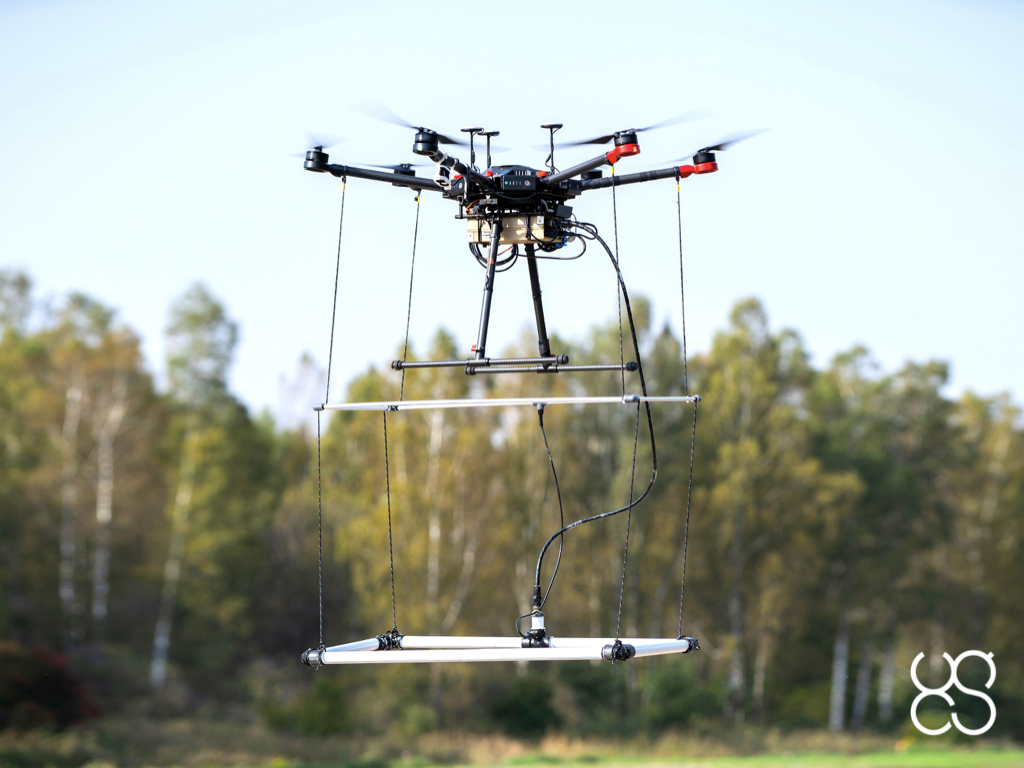
\includegraphics[width=\linewidth]{figs/Huirui/metal_detector_drone.png}
        \caption{UAV-mounted metal detector system\protect\footnotemark.}
        \label{fig:metal_detector_drone}
    \end{subfigure}
    \hfill
    \begin{subfigure}[b]{0.48\linewidth}
        \centering
        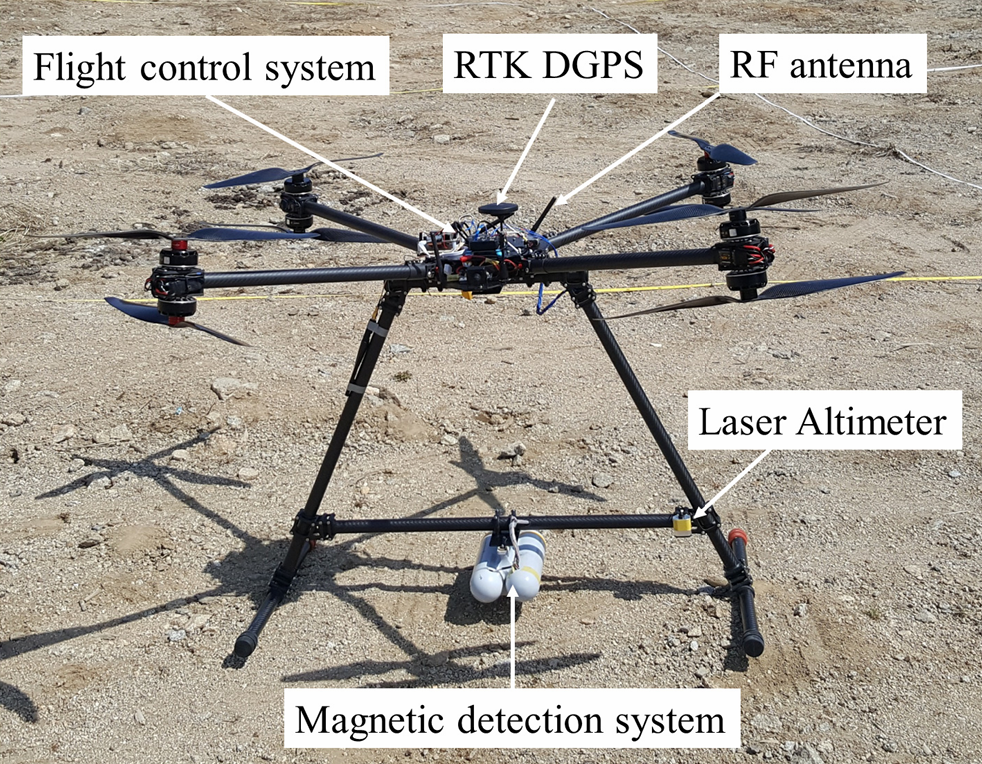
\includegraphics[width=\linewidth]{figs/Huirui/magnetometer_drone.png}
        \caption{Drone-based magnetometer platform~\cite{yoo2020drone}.}
        \label{fig:magnetometer_drone}
    \end{subfigure}
    \caption{Examples of UAV platforms integrating electromagnetic sensors for landmine detection.}
    \label{fig:emi_uav_examples}
\end{figure}

\footnotetext{\url{https://www.sphengineering.com/news/sph-engineering-introduces-the-drone-integrated-metal-detection-system}}

\paragraph{Radiowave and Microwave-Based Systems}

Ground Penetrating Radar (GPR) is a non-invasive geophysical technique that uses electromagnetic waves in the microwave frequency range (typically from several hundred MHz to a few GHz) to detect subsurface anomalies~\cite{gichd2006guidebook}. Unlike EMI-based systems, which respond to conductive or magnetic properties, GPR is sensitive to variations in the dielectric properties of materials~\cite{Gooneratne2004ARO}. It operates by transmitting short-duration radio pulses into the ground via a wideband antenna. When these pulses encounter boundaries between materials with different dielectric constants—such as between soil and a buried landmine—they are partially reflected. The reflected signals are then captured by a receiving antenna, and the time delay and intensity are analyzed to estimate the depth, shape, and dielectric contrast of subsurface targets~\cite{alqudsi2021review, paik2002image}.

As the antenna is moved across the ground, successive measurements are combined to construct two-dimensional slices (radargrams) or even three-dimensional volumetric representations of the subsurface~\cite{Bruschini1997ASO}. The effectiveness of GPR depends heavily on the contrast between the dielectric properties of the object and the surrounding soil. High-frequency systems offer better resolution and are more suited for detecting small anti-personnel mines, while lower-frequency systems provide deeper penetration but at the cost of detail~\cite{gichd2006guidebook}.

\textbf{Strengths:} One of GPR’s major strengths is its ability to detect both metallic and non-metallic mines, including those with plastic casings, by sensing changes in dielectric properties~\cite{Gooneratne2004ARO}. Unlike metal detectors, GPR systems are relatively insensitive to small surface metallic debris, which helps reduce false alarm rates~\cite{gichd2006guidebook}. They also provide useful information about object depth and shape, and can generate cross-sectional or 3D images of the subsurface~\cite{Bruschini1997ASO}. GPR is widely used in archaeological surveys, utility mapping, and geology, and is well understood in terms of commercial deployment and signal processing. Modern GPR systems are compact, lightweight, and pose no radiation hazard due to their low-power operation~\cite{gichd2006guidebook}.

\textbf{Limitations:} The main limitations of GPR lie in its sensitivity to soil conditions. High soil moisture, clay content, or rough surface topology can cause strong attenuation of the radar signal, making it difficult to detect shallow or low-contrast targets~\cite{Gooneratne2004ARO}. Performance can also degrade in dry, homogeneous soils due to insufficient dielectric contrast~\cite{robledo2009survey}. The detection of small anti-personnel mines can be particularly challenging if their signal is masked by surface reflections. Additionally, GPR systems require careful tuning of frequency to balance resolution and penetration depth, and are susceptible to signal distortion caused by subsurface clutter such as rocks, roots, or air pockets~\cite{cardonalandmine}.

\textbf{Drone-Based Applications:} GPR has been widely explored for drone integration due to its capability to detect plastic-cased mines and to provide volumetric subsurface data. UAV-mounted GPR systems typically use lightweight ultra-wideband (UWB) antennas and operate at low altitude to maintain signal fidelity. Applications include detecting anti-tank and anti-personnel mines in varied terrain types, including sand, loam, and clay\footnote{\url{https://www.sphengineering.com/integrated-systems/technologies/gpr}}~\cite{vsipovs2020lightweight,cerquera2017uav,fernandez2018synthetic,amiri2012feasibility,safarov2022detection,vsipovs2020lightweight,colorado2017integrated,schreiber2019advanced,pongrac2022advanced,garcia2020airborne,prager2019application,garcia2019autonomous,burr2018design,fernandez2021development,colorado2017low,lee2023modeling,sipos2017drone,garcia2022safedrone,almutiry2020uav,schartel2018uav,bahnemann2022under,garcia2022validation,chen2023ground}. Figure~\ref{fig:gpr_uav_examples} shows two UAV-based implementations of GPR for landmine detection.

\begin{figure}[h!]
    \centering
    \begin{subfigure}[b]{0.48\linewidth}
        \centering
        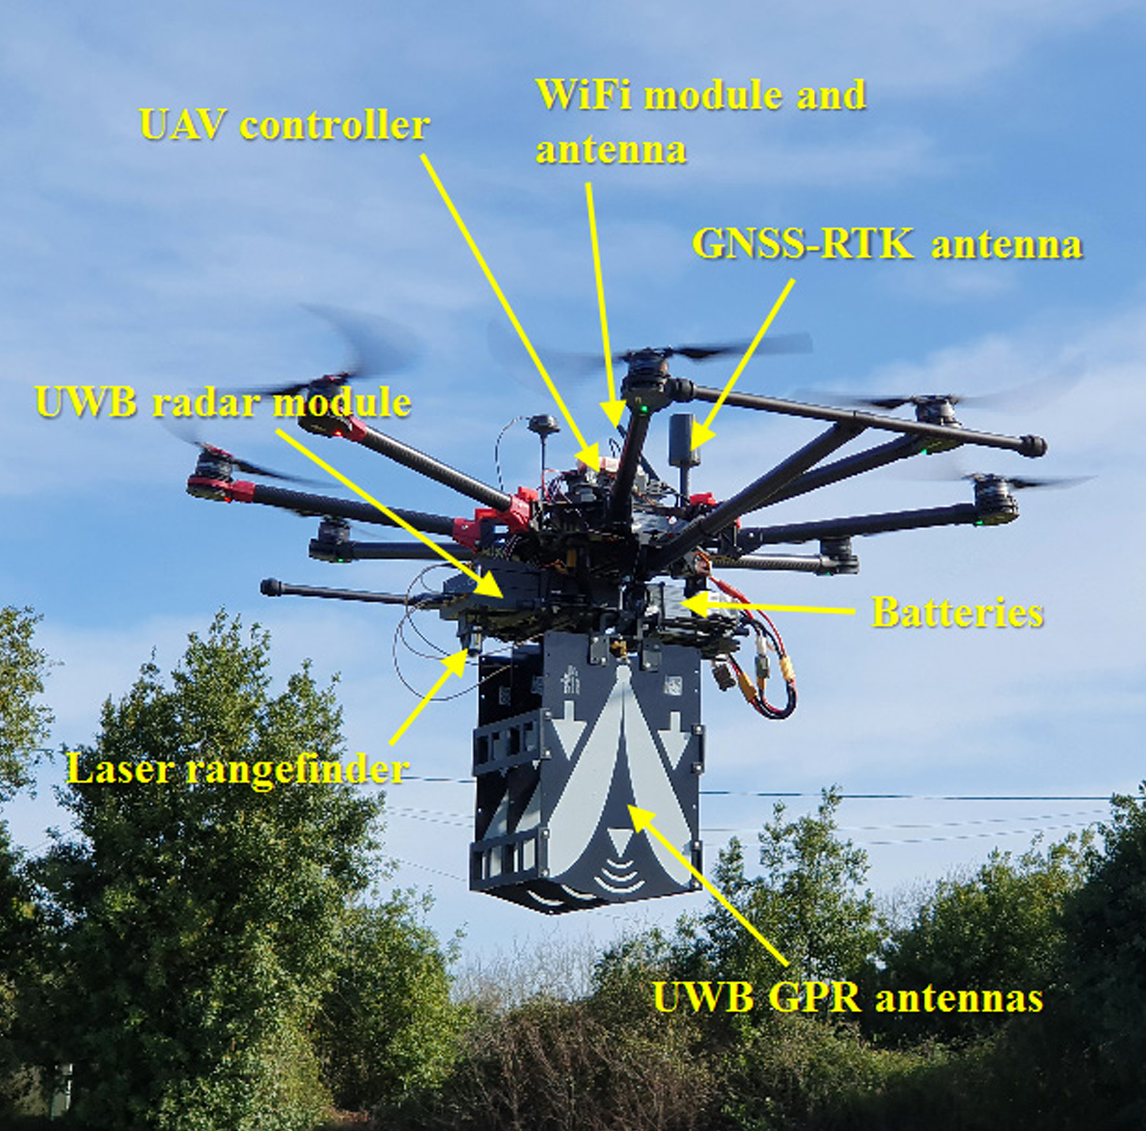
\includegraphics[width=\linewidth]{figs/Huirui/gpr_drone1.png}
        \label{fig:gpr_drone1}
    \end{subfigure}
    \hfill
    \begin{subfigure}[b]{0.48\linewidth}
        \centering
        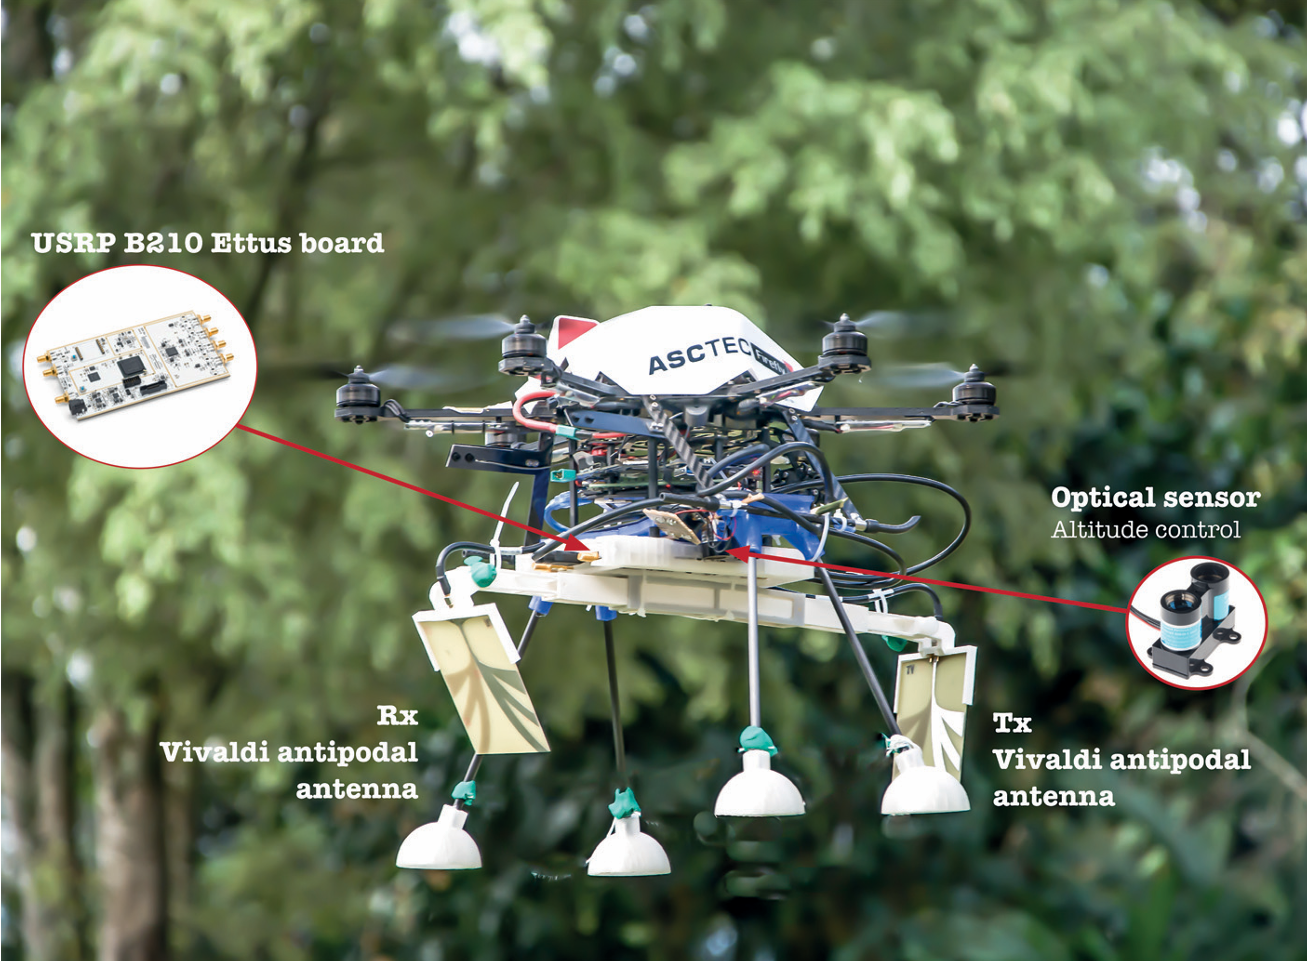
\includegraphics[width=\linewidth]{figs/Huirui/gpr_drone2.png}
        \label{fig:gpr_drone2}
    \end{subfigure}
    \caption{Examples of UAV platforms integrating GPR systems for landmine detection.~\cite{garcia2022safedrone,cerquera2017uav}}
    \label{fig:gpr_uav_examples}
\end{figure}
